\section{Zewnętrzna miara Lebesgue'a w $\Rn$}

Objętość elementarna prostopadłościanów jest intuicyjna i jednoznaczna, jednak jej zasięg ogranicza się do najprostszych figur geometrycznych. Naturalnym pytaniem jest: jak przenieść to pojęcie na dowolne, nawet skrajnie nieregularne podzbiory $\Rn$? Klasyczna próba Jordana — polegająca na przybliżaniu zbiorów skończoną liczbą kostek — okazała się zbyt ciasna, uniemożliwiając zmierzenie choćby zbioru liczb wymiernych. Odpowiedzią Lebesgue’a było dopuszczenie przeliczalnych pokryć kostkami. W ten sposób rodzi się zewnętrzna miara Lebesgue’a $\lambda^{*n}$, która potrafi przypisać wielkość każdemu podzbiorowi przestrzeni, choć ceną za tę uniwersalność jest utrata pełnej addytywności.

\subsection{Pojęcie miary zewnętrznej}

\begin{defi}[Miara zewnętrzna]
    Niech $X$ będzie zbiorem niepustym. Funkcję $\phi \colon \mathcal{P}(X) \to [0, +\infty]$ nazywamy \textbf{miarą zewnętrzną} (w sensie Carathéodory'ego) na $X$, jeżeli spełnia następujące warunki:
    \begin{enumerate}
        \item[(i)] $\phi(\emptyset) = 0$;
        \item[(ii)] \textbf{monotoniczność}: jeżeli $A \subseteq  B \subseteq  X$, to $\phi(A) \mlr \phi(B)$;
        \item[(iii)] \textbf{przeliczalna podaddytywność (subaddytywność)}: dla dowolnego przeliczalnego ciągu podzbiorów $\{A_j\}_{j=1}^\infty \subseteq \mathcal{P}(X)$ zachodzi
              \begin{equation*}
                  \phi\left(\bigcup_{j=1}^\infty A_j\right) \mlr \sum_{j=1}^\infty \phi(A_j).
              \end{equation*}
    \end{enumerate}
\end{defi}
% \begin{wn}[Konstrukcja miary zewnętrznej z funkcji elementarnej]
% Niech $\mathcal{A} \subseteq \mathcal{P}(X)$ będzie dowolną rodziną podzbiorów zawierającą zbiór pusty ($\emptyset \in \mathcal{A}$), a $\alpha \colon \mathcal{A} \to [0, +\infty]$ niech będzie funkcją spełniającą $\alpha(\emptyset) = 0$. Wówczas funkcja $\phi_\alpha \colon \mathcal{P}(X) \to [0, +\infty]$ określona wzorem
% \begin{equation*}
% \phi_\alpha(A) := \inf \left\{ \sum_{j=1}^\infty \alpha(A_j) \colon A_j \in \mathcal{A}, \; A \subseteq \bigcup_{j=1}^\infty A_j \right\} \end{equation*}
% (przyjmując $\inf \emptyset = +\infty$) jest miarą zewnętrzną na $X$. \end{wn}

\subsection{Definicja zewnętrznej miary Lebesgue'a} Stosując powyższą konstrukcję do rodziny kostek w $\Rn$ oraz ich objętości elementarnej $V^n$, otrzymujemy zewnętrzną miarę Lebesgue'a.
\begin{defi}[Zewnętrzna miara Lebesgue'a]
    Dla dowolnego zbioru $A \subseteq \Rn$ jego \textbf{zewnętrzną miarą Lebesgue'a} nazywamy liczbę
    \begin{equation*}
        \lambda^{*}(A) := \inf \left\{ \sum_{j=1}^\infty V^n(P_j) \colon P_j \text{ są kostkami domkniętymi w } \Rn, \; A \subseteq \bigcup_{j=1}^\infty P_j \right\}.
    \end{equation*}
    W literaturze miarę tę oznacza się również przez $L_e^n(A)$ lub $\lambda^*(A)$.
\end{defi}


\begin{figure}
    \centering
    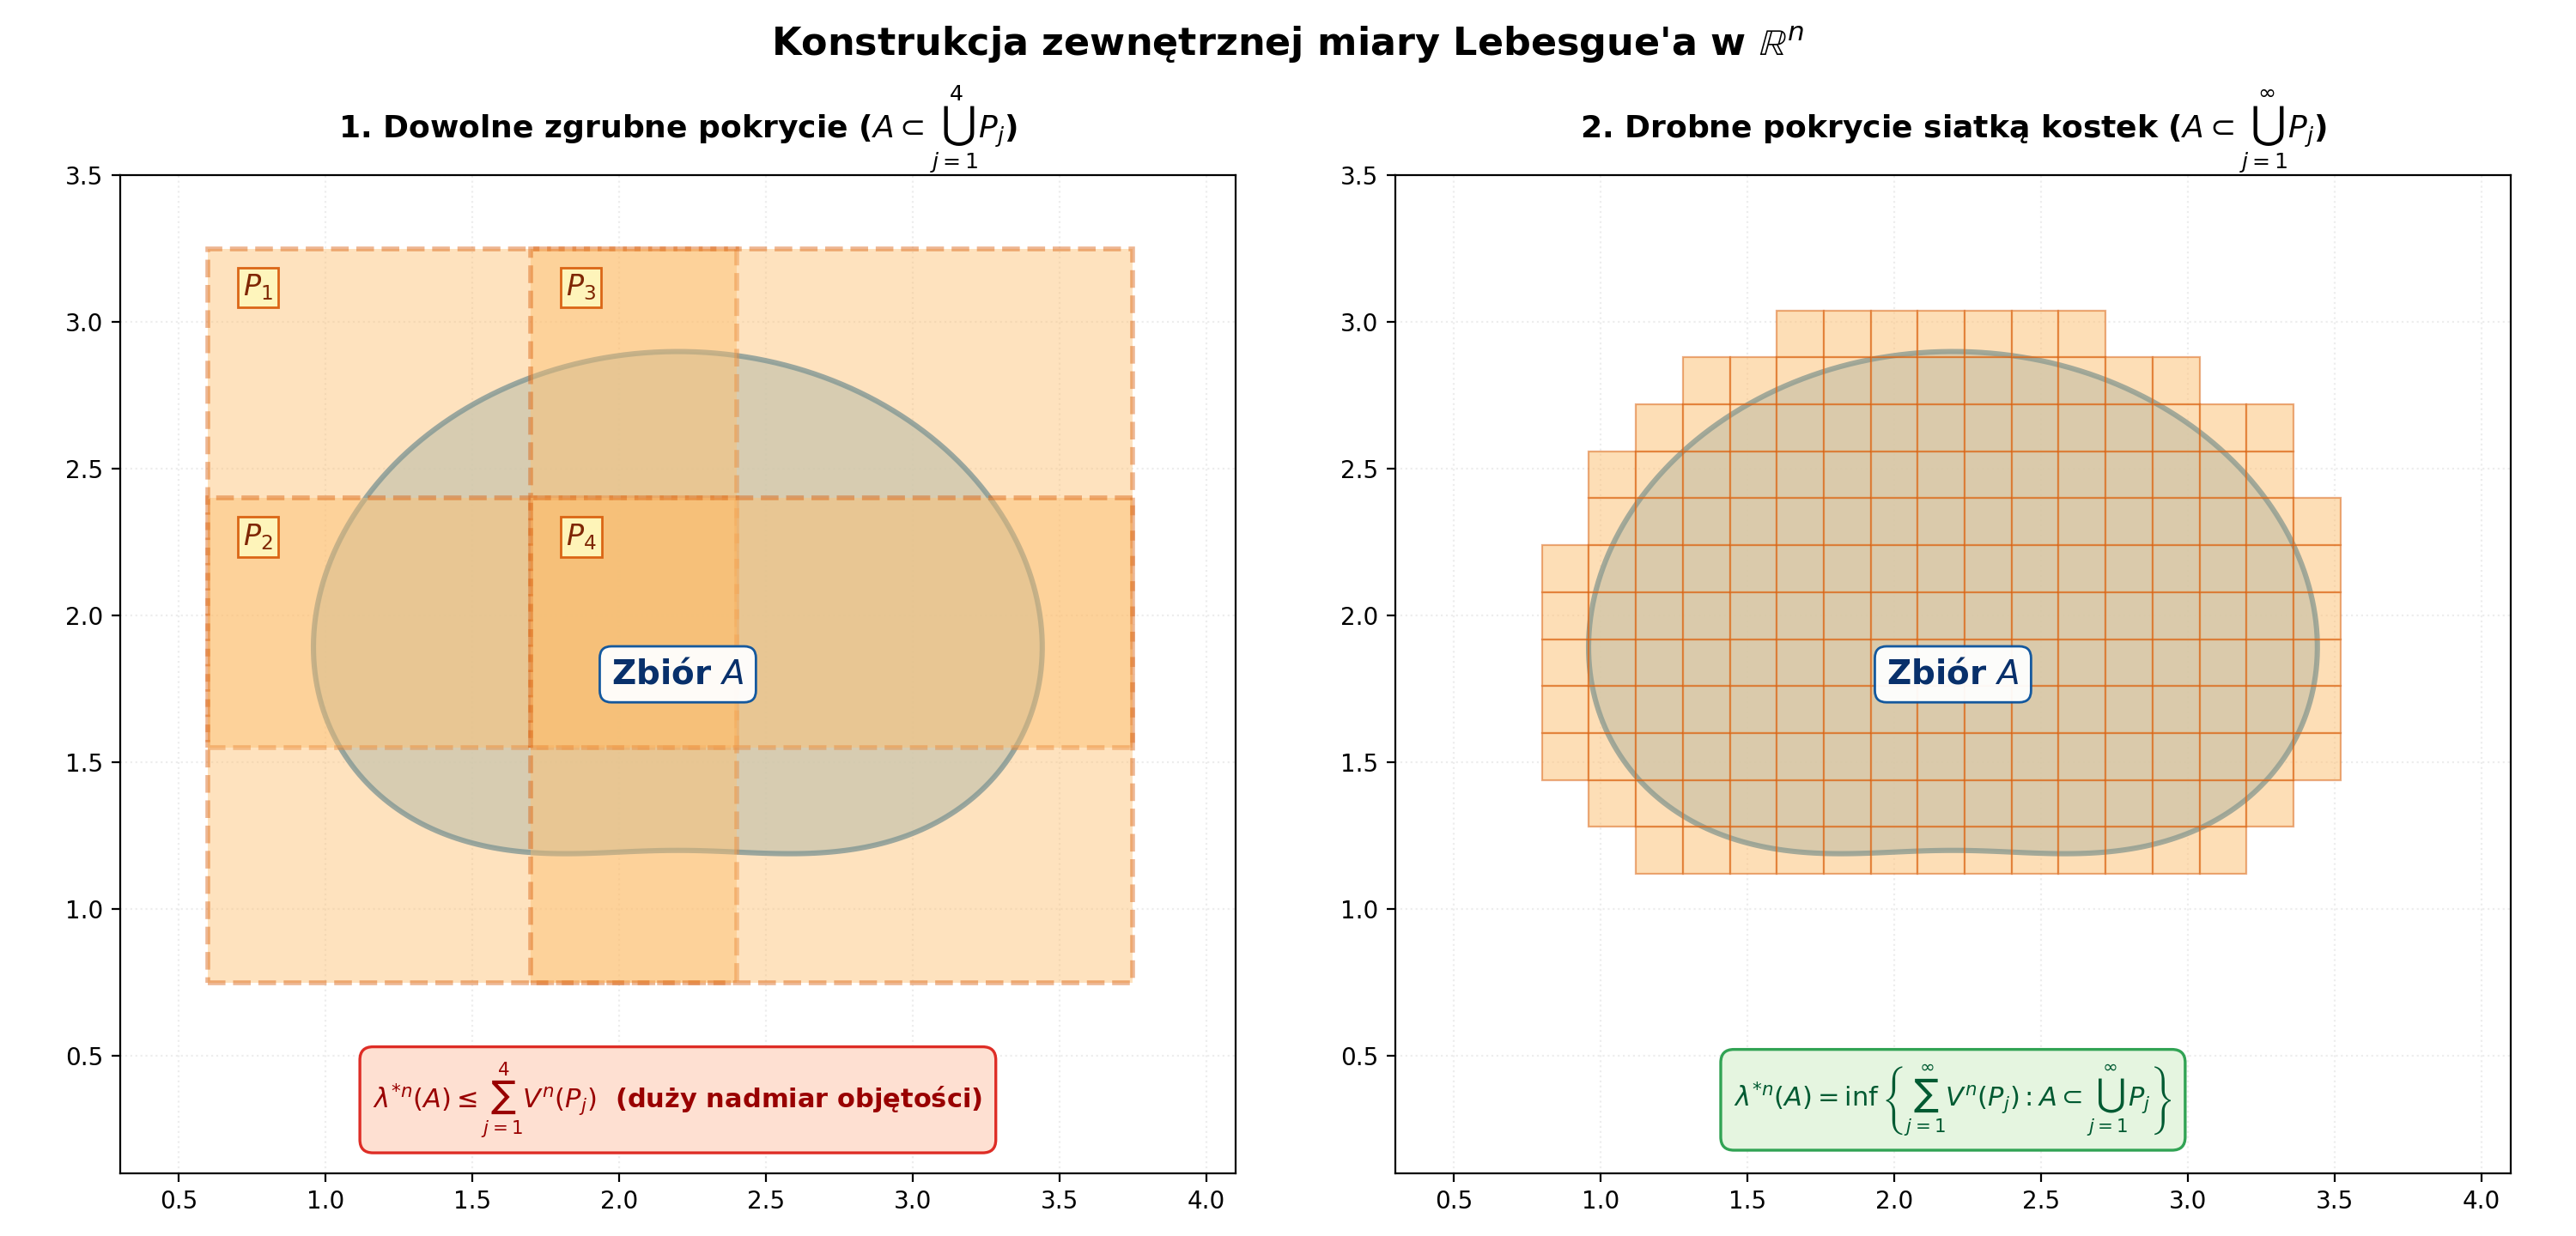
\includegraphics[width=0.5\linewidth]{miara_zewnetrzna_v4.png}
    \caption{Idea konstrukcji zewnętrznej miary Lebesgue'a $\lambda^{*n}(A)$ w $\Rn$: zgrubne pokrycie kostkami z nadmiarem (po lewej) oraz minimalizacja sumy objętości poprzez infimum po coraz drobniejszych pokryciach (po prawej).}
    \label{fig:miara_zewnetrzna}
\end{figure}

\begin{uwaga}[Równoważne warianty pokryć] W definicji zewnętrznej miary Lebesgue'a wartość $\lambda^{*}(A)$ nie ulega zmianie, jeżeli:
    \begin{enumerate}
        \item zamiast kostek domkniętych użyjemy kostek otwartych:
              \begin{equation*} \lambda^{*}(A) = \inf \left\{ \sum_{j=1}^\infty V^n(Q_j) \colon Q_j \text{ są kostkami otwartymi, } A \subseteq \bigcup_{j=1}^\infty Q_j \right\};
              \end{equation*}
        \item ograniczymy się do kostek (otwartych lub domkniętych) o średnicach mniejszych od ustalonej stałej $\delta > 0$, tj. $\diam(P_j) < \delta$.
    \end{enumerate}
\end{uwaga}
\begin{dow}[Uzasadnienie równoważności pokryć otwartych] Niech $\lambda_{\mathrm{open}}^{*}(A)$ oznacza infimum po pokryciach kostkami otwartymi. Ponieważ dla każdej kostki otwartej $Q$ jej domknięcie $\overline{Q}$ jest kostką domkniętą o tej samej objętości ($V^n(\overline{Q}) = V^n(Q)$), każde pokrycie kostkami otwartymi generuje dopuszczalne pokrycie kostkami domkniętymi, skąd $\lambda^{*}(A) \mlr \lambda_{\mathrm{open}}^{n}(A)$.
    W drugą stronę: niech $\{P_j\}_{j=1}^\infty$ będzie pokryciem zbioru $A$ kostkami domkniętymi takim, że
    \begin{equation*}
        \sum_{j=1}^\infty V^n(P_j) \mlr \lambda^{*}(A) + \frac{\varepsilon}{2}.
    \end{equation*}
    Dla każdego $j \in \mathbb{N}$ wybierzmy kostkę otwartą $Q_j \supset P_j$ taką, że $V^n(Q_j) < V^n(P_j) + \varepsilon \cdot 2^{-j-1}$. Wówczas $A \subseteq \bigcup_{j=1}^\infty Q_j$ oraz
    \begin{equation*} \sum_{j=1}^\infty V^n(Q_j) \mlr \sum_{j=1}^\infty V^n(P_j) + \frac{\varepsilon}{2} \sum_{j=1}^\infty 2^{-j} \mlr \lambda^{*}(A) + \varepsilon.
    \end{equation*}
    Z dowolności $\varepsilon > 0$ wynika, że $\lambda_{\mathrm{open}}^{*}(A) \mlr \lambda^{*}(A)$, co daje żądaną równość.
\end{dow}

\subsection{Zgodność z objętością elementarną kostki}
Fundamentalnym faktem teorii jest to, że zewnętrzna miara Lebesgue'a przypisuje każdej kostce jej geometryczną objętość.
\begin{tw}[Objętość kostki a miara zewnętrzna] Dla dowolnej kostki $P \subseteq \Rn$ (domkniętej, otwartej lub częściowo domkniętej) zachodzi tożsamość: \begin{equation*} \lambda^{*}(P) = V^n(P). \end{equation*} \end{tw}
\begin{dow} Wykażemy twierdzenie w dwóch etapach.
    \paragraph{Krok 1: Nierówność $\lambda^{*}(P) \mlr V^n(P)$.} Dla dowolnej kostki $P$ możemy dobrać ciąg kostek domkniętych, w którym pierwszą jest $\overline{P}$, a pozostałe są puste (lub o zerowej objętości). Wówczas $P \subseteq  \overline{P}$, skąd bezpośrednio z definicji infimum otrzymujemy $\lambda^{*}(P) \mlr V^n(\overline{P}) = V^n(P)$.
    \paragraph{Krok 2: Nierówność $V^n(P) \mlr \lambda^{*}(P)$.} Niech $\{Q_j\}_{j=1}^\infty$ będzie dowolnym przeliczalnym pokryciem kostki $P$ kostkami otwartymi, tj. $P \subseteq \bigcup_{j=1}^\infty Q_j$. Ustalmy dowolne $\varepsilon > 0$. Wewnątrz kostki $P$ możemy wybrać kostkę zwartą (domkniętą i ograniczoną) $P_0 \subseteq  P$ taką, że:
    \begin{equation*}
        V^n(P) - \varepsilon < V^n(P_0).
    \end{equation*}

    Ponieważ $P_0 \subseteq  P \subseteq  \bigcup_{j=1}^\infty Q_j$, rodzina $\{Q_j\}_{j=1}^\infty$ stanowi otwarte pokrycie zbioru zwartego $P_0$. Na mocy twierdzenia Heinego-Borela istnieje wskaźnik $N \in \mathbb{N}$ taki, że \begin{equation*} P_0 \subseteq Q_1 \cup Q_2 \cup \dots \cup Q_N. \end{equation*} Ze skończonej podaddytywności elementarnej objętości kostek wynika, że \begin{equation*} V^n(P_0) \mlr \sum_{j=1}^N V^n(Q_j) \mlr \sum_{j=1}^\infty V^n(Q_j). \end{equation*} Łącząc powyższe oszacowania, dostajemy:
    \begin{equation*}
        V^n(P) - \varepsilon < \sum_{j=1}^\infty V^n(Q_j).
    \end{equation*} Przechodząc do infimum po wszystkich możliwych pokryciach kostkami otwartymi, otrzymujemy $V^n(P) - \varepsilon \mlr \lambda^{*}(P)$. Z dowolności $\varepsilon > 0$ wynika nierówność $V^n(P) \mlr \lambda^{*}(P)$, co kończy dowód.
\end{dow}

\subsection{Podstawowe własności analityczne i geometryczne} \begin{tw}[Własności zewnętrznej miary Lebesgue'a]
    Dla dowolnych zbiorów $A, B \subseteq \Rn$, wektora $x_0 \in \Rn$ oraz skalaru $s \in \R$ zachodzą następujące własności:
    \begin{enumerate}
        \item \textbf{Monotoniczność i podaddytywność}: $\lambda^{*}$ jest miarą zewnętrzną na $\mathcal{P}(\Rn)$.
        \item \textbf{Zbiory jednoelementowe i przeliczalne}: dla każdego punktu $x \in \Rn$ zachodzi $\lambda^{*}(\{x\}) = 0$. W konsekwencji dla dowolnego zbioru przeliczalnego $E \subseteq \Rn$ mamy $\lambda^{*}(E) = 0$.
        \item \textbf{Ograniczoność na zbiorach ograniczonych}: jeżeli zbiór $A \subseteq \Rn$ jest ograniczony, to $\lambda^{*}(A) < +\infty$.

        \item \textbf{Niezmienniczość względem translacji}: dla dowolnego przesunięcia $x_0 + A = \{x_0 + x \colon x \in A\}$ zachodzi:
              \begin{equation*}
                  \lambda^{*}(x_0 + A) = \lambda^{*}(A).
              \end{equation*}
        \item \textbf{Jednorodność (skalowanie)}: dla zbioru $sA = \{s \cdot x \colon x \in A\}$ zachodzi:
              \begin{equation*}
                  \lambda^{*}(sA) = |s|^n \lambda^{*}(A).
              \end{equation*}
        \item \textbf{Aproksymacja przez zbiory typu $G_\delta$}: dla każdego zbioru $Y \subseteq \Rn$ istnieje zbiór $G$ typu $G_\delta$ taki, że $Y \subseteq G$ oraz
              \begin{equation*}
                  \lambda^{*}(Y) = \lambda^{*}(G).
              \end{equation*}
              W szczególności $\lambda^{*}$ jest miarą zewnętrzną regularną. \end{enumerate}
\end{tw}
